\documentclass[tikz,border=4pt]{standalone}
\usepackage{amsmath}
\begin{document}
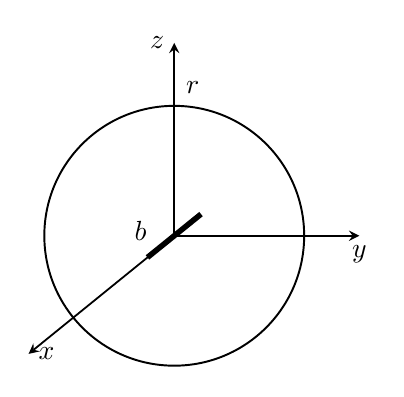
\begin{tikzpicture}[>=stealth, thick, scale=1.0]
  % Sphere of radius r = 1.65
  \draw[line width=0.7pt] (0, 0) circle (1.65);

  % Coordinate axes (x down-left, y right, z up)
  \draw[->, line width=0.65pt] (0, 0) -- (0, 2.45) node[left] {$z$};
  \draw[->, line width=0.65pt] (0, 0) -- (2.35, 0) node[below] {$y$};
  \draw[->, line width=0.65pt] (0, 0) -- (-1.85, -1.50) node[right] {$x$};

  % Oscillation segment along x-axis with amplitude b
  \draw[line width=2.0pt] (0.34, 0.275) -- (-0.34, -0.275);
  \node[left] at (-0.22, 0.06) {$b$};

  % Radius label r on z-axis at sphere intersection
  \node[above right] at (0.02, 1.68) {$r$};
\end{tikzpicture}
\end{document}
